\documentclass{article}\usepackage[]{graphicx}\usepackage[]{color}
% maxwidth is the original width if it is less than linewidth
% otherwise use linewidth (to make sure the graphics do not exceed the margin)
\makeatletter
\def\maxwidth{ %
  \ifdim\Gin@nat@width>\linewidth
    \linewidth
  \else
    \Gin@nat@width
  \fi
}
\makeatother

\definecolor{fgcolor}{rgb}{0.345, 0.345, 0.345}
\newcommand{\hlnum}[1]{\textcolor[rgb]{0.686,0.059,0.569}{#1}}%
\newcommand{\hlstr}[1]{\textcolor[rgb]{0.192,0.494,0.8}{#1}}%
\newcommand{\hlcom}[1]{\textcolor[rgb]{0.678,0.584,0.686}{\textit{#1}}}%
\newcommand{\hlopt}[1]{\textcolor[rgb]{0,0,0}{#1}}%
\newcommand{\hlstd}[1]{\textcolor[rgb]{0.345,0.345,0.345}{#1}}%
\newcommand{\hlkwa}[1]{\textcolor[rgb]{0.161,0.373,0.58}{\textbf{#1}}}%
\newcommand{\hlkwb}[1]{\textcolor[rgb]{0.69,0.353,0.396}{#1}}%
\newcommand{\hlkwc}[1]{\textcolor[rgb]{0.333,0.667,0.333}{#1}}%
\newcommand{\hlkwd}[1]{\textcolor[rgb]{0.737,0.353,0.396}{\textbf{#1}}}%
\let\hlipl\hlkwb

\usepackage{framed}
\makeatletter
\newenvironment{kframe}{%
 \def\at@end@of@kframe{}%
 \ifinner\ifhmode%
  \def\at@end@of@kframe{\end{minipage}}%
  \begin{minipage}{\columnwidth}%
 \fi\fi%
 \def\FrameCommand##1{\hskip\@totalleftmargin \hskip-\fboxsep
 \colorbox{shadecolor}{##1}\hskip-\fboxsep
     % There is no \\@totalrightmargin, so:
     \hskip-\linewidth \hskip-\@totalleftmargin \hskip\columnwidth}%
 \MakeFramed {\advance\hsize-\width
   \@totalleftmargin\z@ \linewidth\hsize
   \@setminipage}}%
 {\par\unskip\endMakeFramed%
 \at@end@of@kframe}
\makeatother

\definecolor{shadecolor}{rgb}{.97, .97, .97}
\definecolor{messagecolor}{rgb}{0, 0, 0}
\definecolor{warningcolor}{rgb}{1, 0, 1}
\definecolor{errorcolor}{rgb}{1, 0, 0}
\newenvironment{knitrout}{}{} % an empty environment to be redefined in TeX

\usepackage{alltt}
\usepackage{rotating}
\usepackage{graphicx, color, framed, alltt}
\usepackage{fullpage}
\usepackage{pdflscape}
\usepackage{placeins}
\usepackage{longtable}
\IfFileExists{upquote.sty}{\usepackage{upquote}}{}
\begin{document}



\section*{Analaysis of Public Housing in County Census Tracts and \\Proximity to CE(s)}

\textbf{Original Analysis}\\
\textbf{By: D. White}\\
\textbf{Date: 2019-11-13}\\
\\
----------------------------\\
\break
KNITR File: Report\textunderscore Logistic\textunderscore Model.Rnw \\
\begin{knitrout}
\definecolor{shadecolor}{rgb}{0.969, 0.969, 0.969}\color{fgcolor}\begin{kframe}
\begin{verbatim}
## [1] "Generated on: 2019-11-19 12:18:28"
\end{verbatim}
\end{kframe}
\end{knitrout}
  





Methods: A multistep data processing routine was performed for each county to integrate spatial and tabular data sets of CE presence/absence and public housing counts at a census tract level in each county. Data were aggregated to the final observed year for each county. Census tract data and HUD data date to 2000. HUD data include Section-8 vouchers and Low-Income Housing Tax Credit (LIHTC) unit counts in each census tract.The final tabular data set for each county is presented in this analysis. A logistic regression was performed on an all county data set to test the probability of a CE located in census tract dependent upon HUD housing counts (Tables 1-3). Tables 4-30 show results of the logistic regression for each individual county. ALB and DGL were not included in the anlaysis due small sample size. CHS is generating an error that I can not solve at this time. The model appears to run correctly in R as a stand-alone, but when output to Latex it generates the error found on page 8. LEB is of particular interest. \\ 

The data processing by county can be found in the path below.\\ 
C:\textbackslash Users\textbackslash whitedl\textbackslash Documents\textbackslash R\textunderscore Code\textbackslash HUD\textunderscore Project\textunderscore Code\textbackslash CNTYNAME\textunderscore Public\textunderscore Housing\textunderscore CE.R\\

Table 1 shows the coefficient estimates and related information that result from fitting a logistic regression to predict the probability of a CE located in a census tract based on the predictors Section 8 and Tax Credit housing counts in the corresponding census tracts. A positive coefficent will indicate that an increase in public housing is associated with an increase in the probability of a CE in a given Census Tract. A negative coefficent will imply that increased numbers of public housing units are associated with a decreased probability of a CE in a census tract. A highly significant negative effect is observed for Section 8 housing (P$<$.01) while a positive significant effect (P$<$.05) is observed for Tax Credit housing.\\

Table 2 reports a NULL model deviance of 1093. A residual deviance of 1032 is observed.\\ 

A McFadden statistic is reported in table 3. The McFadden statisitic is complementary to a linear regression R2 value. A value of 0.068 indicates a relatively poor model fit. Although not as severe if it were an OLS R2 value.\\  

Observations: 1. Many zeros are present in the Tax Credit housing. Originally, these were coded as NA, but that was an error. 2. I examined other model derivatives such as each predictor alone and an interaction effect. Those other models were even less compelling. 3. Overall, I do not find this to be a strong model. But my limited experience with logistic/categorical modeling could be an issue. 


\pagebreak
\newpage
\FloatBarrier

\begin{knitrout}
\definecolor{shadecolor}{rgb}{0.969, 0.969, 0.969}\color{fgcolor}\begin{figure}
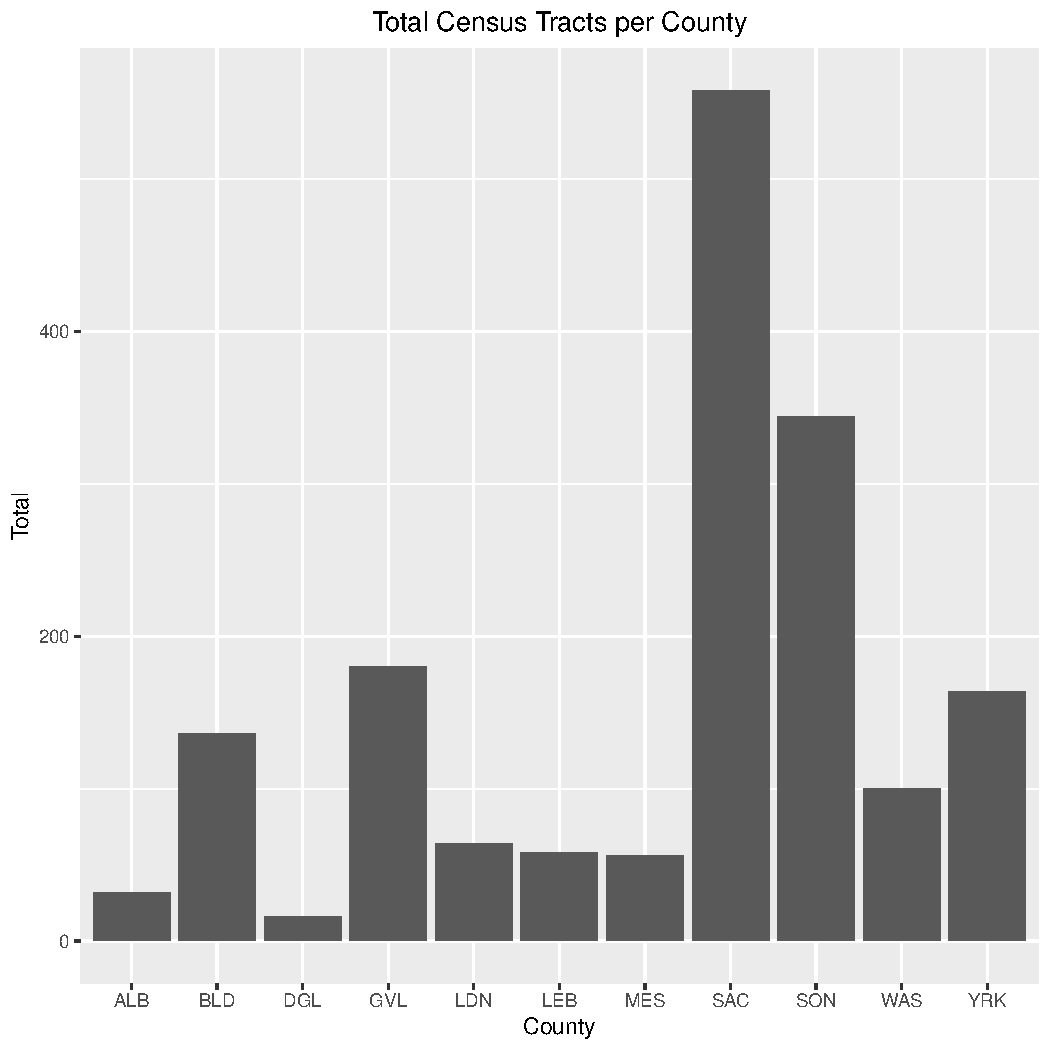
\includegraphics[width=\maxwidth]{figure/Bar_All_Counties_Tract-1} \caption[Total Census Tracts by County]{Total Census Tracts by County}\label{fig:Bar_All_Counties_Tract}
\end{figure}


\end{knitrout}


\begin{knitrout}
\definecolor{shadecolor}{rgb}{0.969, 0.969, 0.969}\color{fgcolor}\begin{figure}
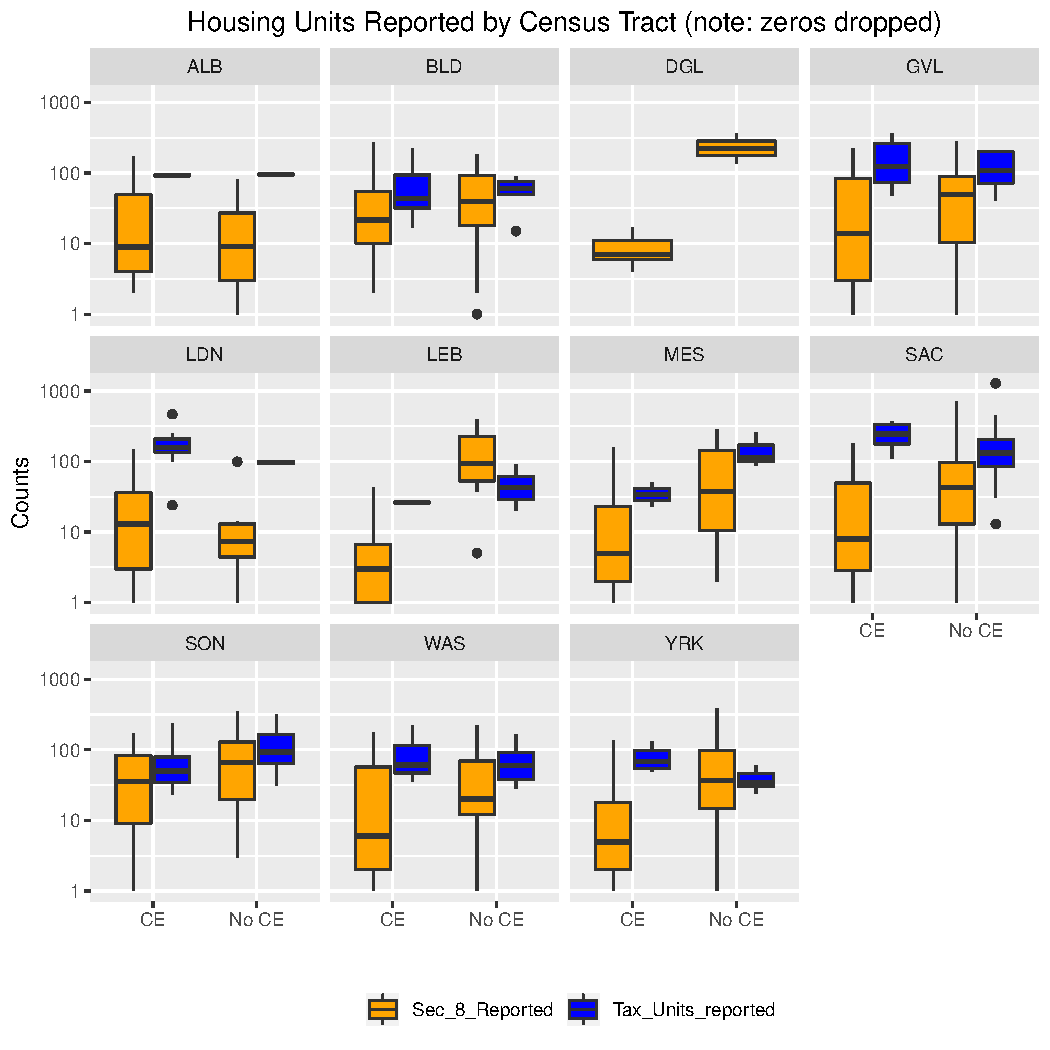
\includegraphics[width=\maxwidth]{figure/BoxPlot_All_Units-1} \caption[Housing Units Reported by Census Tract]{Housing Units Reported by Census Tract}\label{fig:BoxPlot_All_Units}
\end{figure}


\end{knitrout}


\begin{knitrout}
\definecolor{shadecolor}{rgb}{0.969, 0.969, 0.969}\color{fgcolor}\begin{figure}
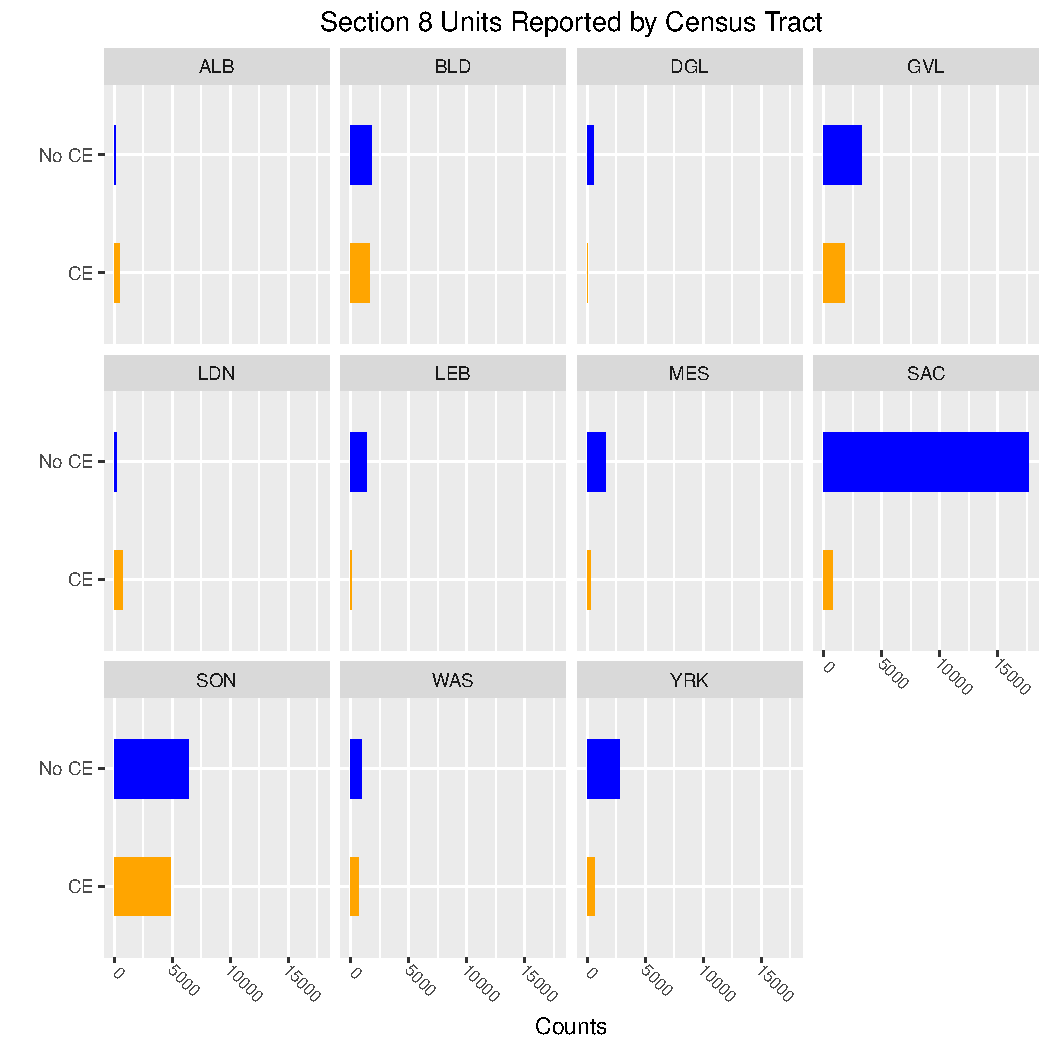
\includegraphics[width=\maxwidth]{figure/MultiPlot_SEC_8_Counts-1} \caption[Section 8 Units Reported by Census Tract]{Section 8 Units Reported by Census Tract}\label{fig:MultiPlot_SEC_8_Counts}
\end{figure}


\end{knitrout}


\begin{knitrout}
\definecolor{shadecolor}{rgb}{0.969, 0.969, 0.969}\color{fgcolor}\begin{figure}
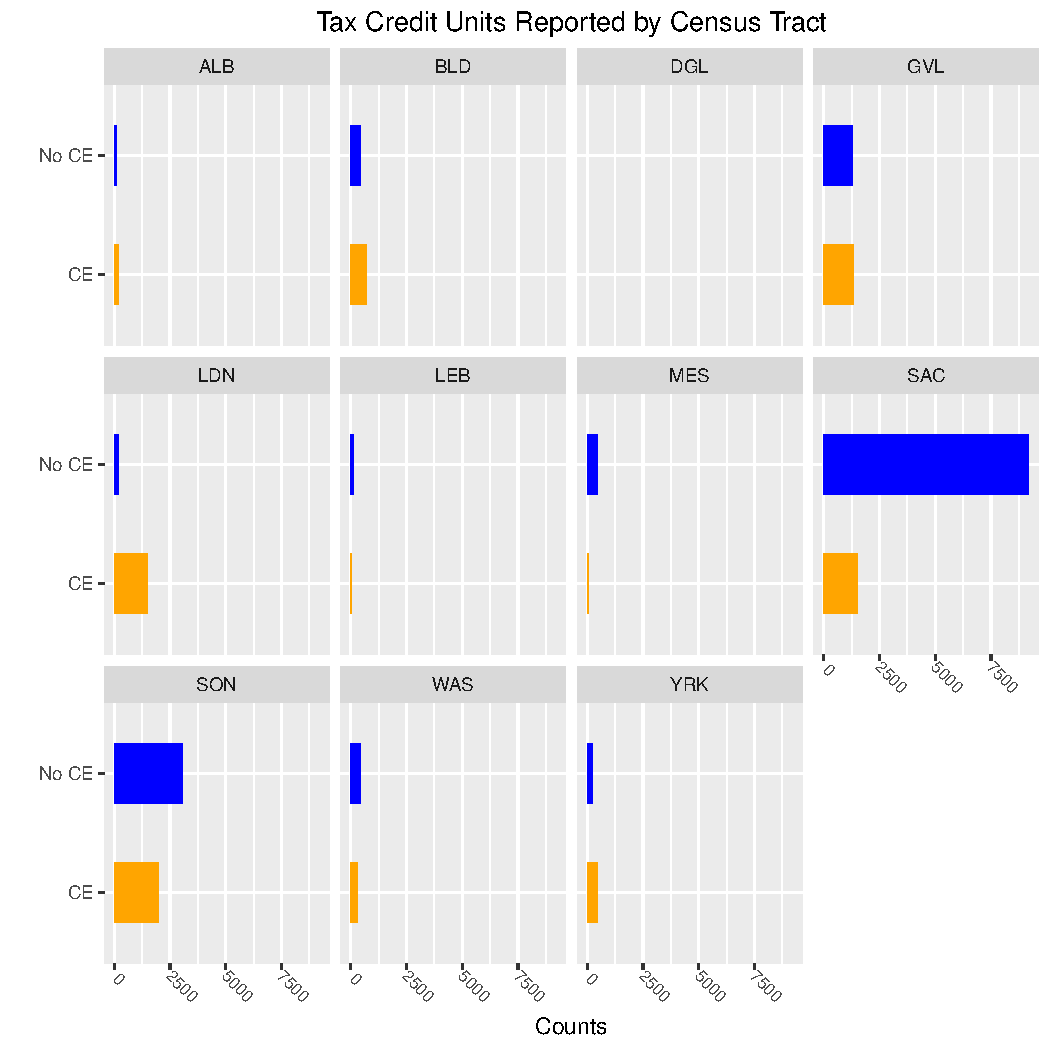
\includegraphics[width=\maxwidth]{figure/MultiPlot_Tax_Units_Counts-1} \caption[Tax Credit Units Reported by Census Tract]{Tax Credit Units Reported by Census Tract}\label{fig:MultiPlot_Tax_Units_Counts}
\end{figure}


\end{knitrout}

\begin{knitrout}
\definecolor{shadecolor}{rgb}{0.969, 0.969, 0.969}\color{fgcolor}\begin{figure}
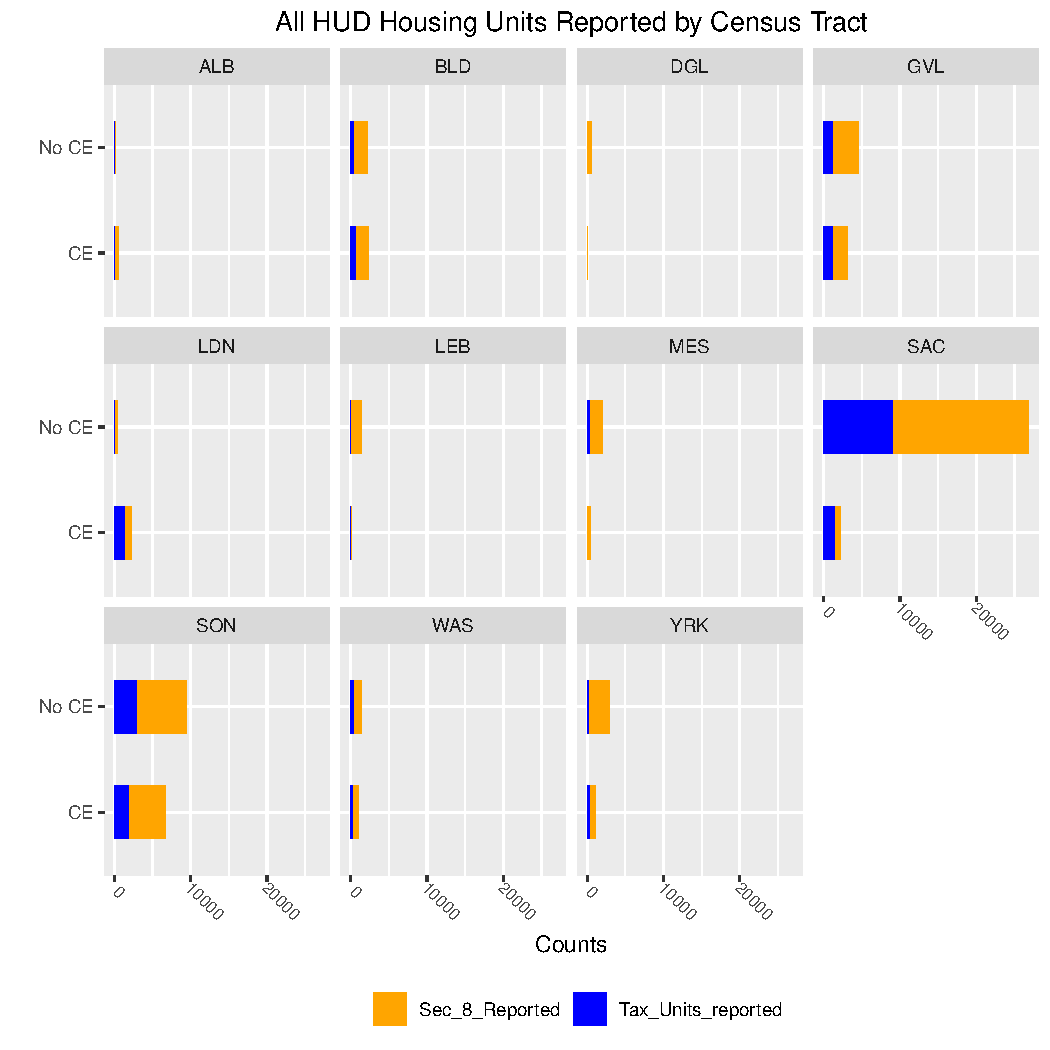
\includegraphics[width=\maxwidth]{figure/MultiPlot_All_Units_Counts_stacked-1} \caption[Housing Units Reported by Census Tract]{Housing Units Reported by Census Tract}\label{fig:MultiPlot_All_Units_Counts_stacked}
\end{figure}


\end{knitrout}


\begin{knitrout}
\definecolor{shadecolor}{rgb}{0.969, 0.969, 0.969}\color{fgcolor}\begin{figure}
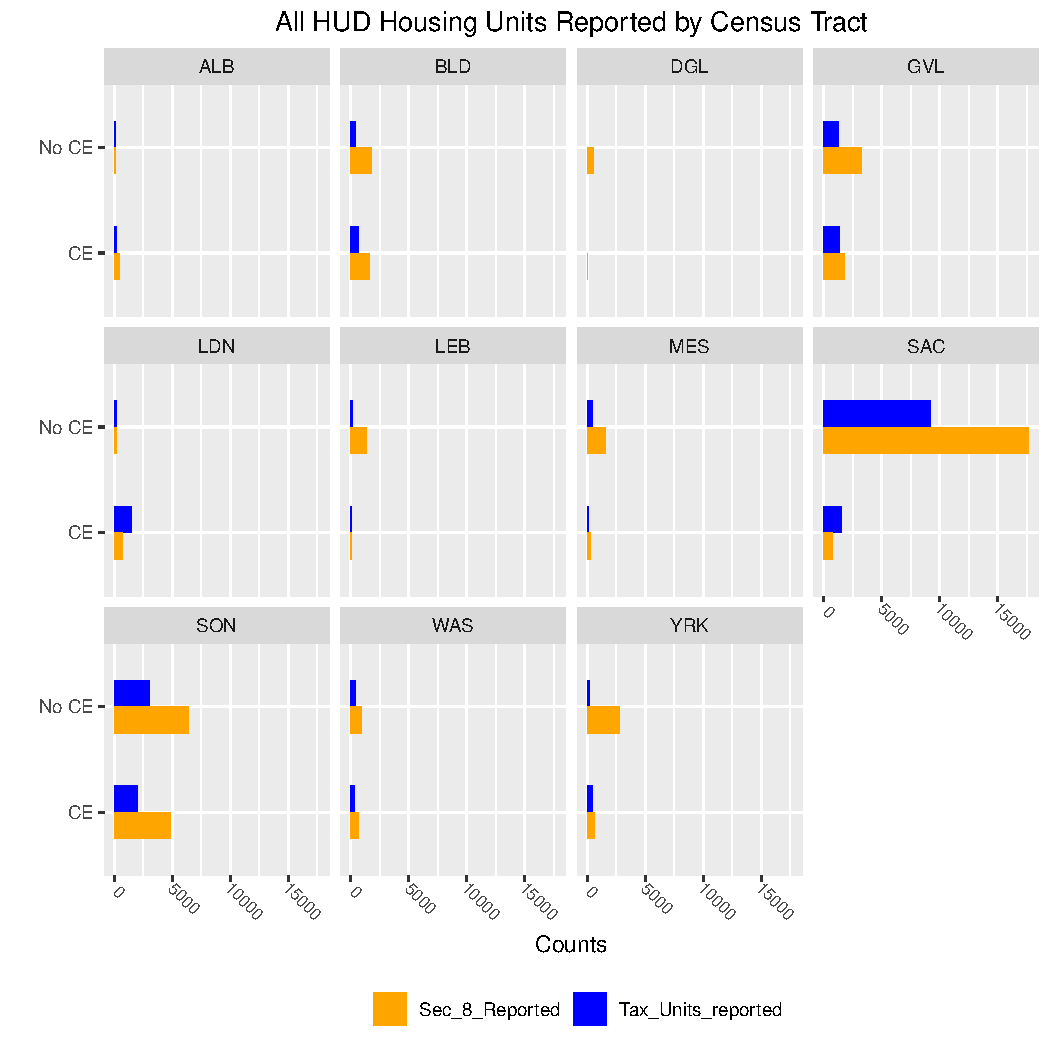
\includegraphics[width=\maxwidth]{figure/MultiPlot_All_Units_Counts_dodge-1} \caption[Housing Units Reported by Census Tract]{Housing Units Reported by Census Tract}\label{fig:MultiPlot_All_Units_Counts_dodge}
\end{figure}


\end{knitrout}

\newpage

\FloatBarrier


% Table created by stargazer v.5.2.2 by Marek Hlavac, Harvard University. E-mail: hlavac at fas.harvard.edu
% Date and time: Tue, Nov 19, 2019 - 12:18:43 PM
% Requires LaTeX packages: dcolumn 
\begin{table}[!htbp] \centering 
  \caption{All Counties: Regression Results: HUD Housing} 
  \label{} 
\begin{tabular}{@{\extracolsep{5pt}}lD{.}{.}{-3} } 
\\[-1.8ex]\hline 
\hline \\[-1.8ex] 
 & \multicolumn{1}{c}{\textit{Dependent variable:}} \\ 
\cline{2-2} 
\\[-1.8ex] & \multicolumn{1}{c}{CE\_Present} \\ 
\hline \\[-1.8ex] 
 Sec\_8\_Reported & -0.010^{***} \\ 
  & (0.002) \\ 
  & \\ 
 Tax\_Units\_reported & 0.003^{**} \\ 
  & (0.001) \\ 
  & \\ 
 Constant & -0.063 \\ 
  & (0.093) \\ 
  & \\ 
\hline \\[-1.8ex] 
Observations & \multicolumn{1}{c}{846} \\ 
Log Likelihood & \multicolumn{1}{c}{-537.417} \\ 
Akaike Inf. Crit. & \multicolumn{1}{c}{1,080.834} \\ 
\hline 
\hline \\[-1.8ex] 
\textit{Note:}  & \multicolumn{1}{r}{$^{*}$p$<$0.1; $^{**}$p$<$0.05; $^{***}$p$<$0.01} \\ 
\end{tabular} 
\end{table} 



% Table created by stargazer v.5.2.2 by Marek Hlavac, Harvard University. E-mail: hlavac at fas.harvard.edu
% Date and time: Tue, Nov 19, 2019 - 12:18:43 PM
% Requires LaTeX packages: dcolumn 
\begin{table}[!htbp] \centering 
  \caption{All Counties: Analysis of Deviance} 
  \label{} 
\begin{tabular}{@{\extracolsep{5pt}}lD{.}{.}{-3} D{.}{.}{-3} D{.}{.}{-3} D{.}{.}{-3} D{.}{.}{-3} D{.}{.}{-3} D{.}{.}{-3} } 
\\[-1.8ex]\hline 
\hline \\[-1.8ex] 
Statistic & \multicolumn{1}{c}{N} & \multicolumn{1}{c}{Mean} & \multicolumn{1}{c}{St. Dev.} & \multicolumn{1}{c}{Min} & \multicolumn{1}{c}{Pctl(25)} & \multicolumn{1}{c}{Pctl(75)} & \multicolumn{1}{c}{Max} \\ 
\hline \\[-1.8ex] 
Df & 2 & 1.000 & 0.000 & 1.000 & 1.000 & 1.000 & 1.000 \\ 
Deviance & 2 & 26.543 & 29.441 & 5.725 & 16.134 & 36.952 & 47.360 \\ 
Resid. Df & 3 & 844.000 & 1.000 & 843 & 843.5 & 844.5 & 845 \\ 
Resid. Dev & 3 & 1,094.438 & 29.137 & 1,074.834 & 1,077.697 & 1,104.239 & 1,127.920 \\ 
Pr(\textgreater Chi) & 2 & 0.008 & 0.012 & 0.000 & 0.004 & 0.013 & 0.017 \\ 
\hline \\[-1.8ex] 
\end{tabular} 
\end{table} 



% Table created by stargazer v.5.2.2 by Marek Hlavac, Harvard University. E-mail: hlavac at fas.harvard.edu
% Date and time: Tue, Nov 19, 2019 - 12:18:43 PM
% Requires LaTeX packages: dcolumn 
\begin{table}[!htbp] \centering 
  \caption{All Counties: McFadden Statistic:similar to R2} 
  \label{} 
\begin{tabular}{@{\extracolsep{5pt}} D{.}{.}{-3} D{.}{.}{-3} D{.}{.}{-3} D{.}{.}{-3} D{.}{.}{-3} D{.}{.}{-3} } 
\\[-1.8ex]\hline 
\hline \\[-1.8ex] 
\multicolumn{1}{c}{llh} & \multicolumn{1}{c}{llhNull} & \multicolumn{1}{c}{G2} & \multicolumn{1}{c}{McFadden} & \multicolumn{1}{c}{r2ML} & \multicolumn{1}{c}{r2CU} \\ 
\hline \\[-1.8ex] 
-537.417 & -570.634 & 66.433 & 0.058 & 0.076 & 0.102 \\ 
\hline \\[-1.8ex] 
\end{tabular} 
\end{table} 



% Table created by stargazer v.5.2.2 by Marek Hlavac, Harvard University. E-mail: hlavac at fas.harvard.edu
% Date and time: Tue, Nov 19, 2019 - 12:18:43 PM
% Requires LaTeX packages: dcolumn 
\begin{table}[!htbp] \centering 
  \caption{BLD Regression Results: HUD Housing} 
  \label{} 
\begin{tabular}{@{\extracolsep{5pt}}lD{.}{.}{-3} } 
\\[-1.8ex]\hline 
\hline \\[-1.8ex] 
 & \multicolumn{1}{c}{\textit{Dependent variable:}} \\ 
\cline{2-2} 
\\[-1.8ex] & \multicolumn{1}{c}{CE\_Present} \\ 
\hline \\[-1.8ex] 
 Sec\_8\_Reported & -0.010^{*} \\ 
  & (0.006) \\ 
  & \\ 
 Tax\_Units\_reported & 0.013 \\ 
  & (0.009) \\ 
  & \\ 
 Constant & 0.480 \\ 
  & (0.336) \\ 
  & \\ 
\hline \\[-1.8ex] 
Observations & \multicolumn{1}{c}{68} \\ 
Log Likelihood & \multicolumn{1}{c}{-44.997} \\ 
Akaike Inf. Crit. & \multicolumn{1}{c}{95.995} \\ 
\hline 
\hline \\[-1.8ex] 
\textit{Note:}  & \multicolumn{1}{r}{$^{*}$p$<$0.1; $^{**}$p$<$0.05; $^{***}$p$<$0.01} \\ 
\end{tabular} 
\end{table} 



% Table created by stargazer v.5.2.2 by Marek Hlavac, Harvard University. E-mail: hlavac at fas.harvard.edu
% Date and time: Tue, Nov 19, 2019 - 12:18:43 PM
% Requires LaTeX packages: dcolumn 
\begin{table}[!htbp] \centering 
  \caption{BLD: Analysis of Deviance} 
  \label{} 
\begin{tabular}{@{\extracolsep{5pt}}lD{.}{.}{-3} D{.}{.}{-3} D{.}{.}{-3} D{.}{.}{-3} D{.}{.}{-3} D{.}{.}{-3} D{.}{.}{-3} } 
\\[-1.8ex]\hline 
\hline \\[-1.8ex] 
Statistic & \multicolumn{1}{c}{N} & \multicolumn{1}{c}{Mean} & \multicolumn{1}{c}{St. Dev.} & \multicolumn{1}{c}{Min} & \multicolumn{1}{c}{Pctl(25)} & \multicolumn{1}{c}{Pctl(75)} & \multicolumn{1}{c}{Max} \\ 
\hline \\[-1.8ex] 
Df & 2 & 1.000 & 0.000 & 1.000 & 1.000 & 1.000 & 1.000 \\ 
Deviance & 2 & 1.872 & 0.683 & 1.388 & 1.630 & 2.113 & 2.355 \\ 
Resid. Df & 3 & 66.000 & 1.000 & 65 & 65.5 & 66.5 & 67 \\ 
Resid. Dev & 3 & 92.027 & 1.892 & 89.995 & 91.172 & 93.044 & 93.738 \\ 
Pr(\textgreater Chi) & 2 & 0.182 & 0.080 & 0.125 & 0.153 & 0.210 & 0.239 \\ 
\hline \\[-1.8ex] 
\end{tabular} 
\end{table} 



% Table created by stargazer v.5.2.2 by Marek Hlavac, Harvard University. E-mail: hlavac at fas.harvard.edu
% Date and time: Tue, Nov 19, 2019 - 12:18:43 PM
% Requires LaTeX packages: dcolumn 
\begin{table}[!htbp] \centering 
  \caption{BLD: McFadden Statistic:similar to R2} 
  \label{} 
\begin{tabular}{@{\extracolsep{5pt}} D{.}{.}{-3} D{.}{.}{-3} D{.}{.}{-3} D{.}{.}{-3} D{.}{.}{-3} D{.}{.}{-3} } 
\\[-1.8ex]\hline 
\hline \\[-1.8ex] 
\multicolumn{1}{c}{llh} & \multicolumn{1}{c}{llhNull} & \multicolumn{1}{c}{G2} & \multicolumn{1}{c}{McFadden} & \multicolumn{1}{c}{r2ML} & \multicolumn{1}{c}{r2CU} \\ 
\hline \\[-1.8ex] 
-44.997 & -46.869 & 3.743 & 0.040 & 0.054 & 0.072 \\ 
\hline \\[-1.8ex] 
\end{tabular} 
\end{table} 




\begin{kframe}


{\ttfamily\noindent\bfseries\color{errorcolor}{\#\# Error in family\$linkfun(mustart): Argument mu must be a nonempty numeric vector}}

{\ttfamily\noindent\bfseries\color{errorcolor}{\#\# Error in .stargazer.wrap(..., type = type, title = title, style = style, : object 'CHS\_model1' not found}}\end{kframe}

\begin{kframe}


{\ttfamily\noindent\bfseries\color{errorcolor}{\#\# Error in anova(CHS\_model1, test = "{}Chisq"{}): object 'CHS\_model1' not found}}

{\ttfamily\noindent\bfseries\color{errorcolor}{\#\# Error in .stargazer.wrap(..., type = type, title = title, style = style, : object 'CHS\_model\_anova' not found}}\end{kframe}

\begin{kframe}


{\ttfamily\noindent\bfseries\color{errorcolor}{\#\# Error in pR2(CHS\_model1): object 'CHS\_model1' not found}}

{\ttfamily\noindent\bfseries\color{errorcolor}{\#\# Error in .stargazer.wrap(..., type = type, title = title, style = style, : object 'CHS\_model\_pR2' not found}}\end{kframe}



% Table created by stargazer v.5.2.2 by Marek Hlavac, Harvard University. E-mail: hlavac at fas.harvard.edu
% Date and time: Tue, Nov 19, 2019 - 12:18:43 PM
% Requires LaTeX packages: dcolumn 
\begin{table}[!htbp] \centering 
  \caption{GVL Regression Results: HUD Housing} 
  \label{} 
\begin{tabular}{@{\extracolsep{5pt}}lD{.}{.}{-3} } 
\\[-1.8ex]\hline 
\hline \\[-1.8ex] 
 & \multicolumn{1}{c}{\textit{Dependent variable:}} \\ 
\cline{2-2} 
\\[-1.8ex] & \multicolumn{1}{c}{CE\_Present} \\ 
\hline \\[-1.8ex] 
 Sec\_8\_Reported & -0.006 \\ 
  & (0.004) \\ 
  & \\ 
 Tax\_Units\_reported & 0.005 \\ 
  & (0.004) \\ 
  & \\ 
 Constant & -0.143 \\ 
  & (0.274) \\ 
  & \\ 
\hline \\[-1.8ex] 
Observations & \multicolumn{1}{c}{90} \\ 
Log Likelihood & \multicolumn{1}{c}{-59.773} \\ 
Akaike Inf. Crit. & \multicolumn{1}{c}{125.546} \\ 
\hline 
\hline \\[-1.8ex] 
\textit{Note:}  & \multicolumn{1}{r}{$^{*}$p$<$0.1; $^{**}$p$<$0.05; $^{***}$p$<$0.01} \\ 
\end{tabular} 
\end{table} 



% Table created by stargazer v.5.2.2 by Marek Hlavac, Harvard University. E-mail: hlavac at fas.harvard.edu
% Date and time: Tue, Nov 19, 2019 - 12:18:43 PM
% Requires LaTeX packages: dcolumn 
\begin{table}[!htbp] \centering 
  \caption{GVL: Analysis of Deviance} 
  \label{} 
\begin{tabular}{@{\extracolsep{5pt}}lD{.}{.}{-3} D{.}{.}{-3} D{.}{.}{-3} D{.}{.}{-3} D{.}{.}{-3} D{.}{.}{-3} D{.}{.}{-3} } 
\\[-1.8ex]\hline 
\hline \\[-1.8ex] 
Statistic & \multicolumn{1}{c}{N} & \multicolumn{1}{c}{Mean} & \multicolumn{1}{c}{St. Dev.} & \multicolumn{1}{c}{Min} & \multicolumn{1}{c}{Pctl(25)} & \multicolumn{1}{c}{Pctl(75)} & \multicolumn{1}{c}{Max} \\ 
\hline \\[-1.8ex] 
Df & 2 & 1.000 & 0.000 & 1.000 & 1.000 & 1.000 & 1.000 \\ 
Deviance & 2 & 1.517 & 0.530 & 1.143 & 1.330 & 1.704 & 1.892 \\ 
Resid. Df & 3 & 88.000 & 1.000 & 87 & 87.5 & 88.5 & 89 \\ 
Resid. Dev & 3 & 121.188 & 1.532 & 119.546 & 120.491 & 122.009 & 122.580 \\ 
Pr(\textgreater Chi) & 2 & 0.227 & 0.082 & 0.169 & 0.198 & 0.256 & 0.285 \\ 
\hline \\[-1.8ex] 
\end{tabular} 
\end{table} 



% Table created by stargazer v.5.2.2 by Marek Hlavac, Harvard University. E-mail: hlavac at fas.harvard.edu
% Date and time: Tue, Nov 19, 2019 - 12:18:43 PM
% Requires LaTeX packages: dcolumn 
\begin{table}[!htbp] \centering 
  \caption{GVL: McFadden Statistic:similar to R2} 
  \label{} 
\begin{tabular}{@{\extracolsep{5pt}} D{.}{.}{-3} D{.}{.}{-3} D{.}{.}{-3} D{.}{.}{-3} D{.}{.}{-3} D{.}{.}{-3} } 
\\[-1.8ex]\hline 
\hline \\[-1.8ex] 
\multicolumn{1}{c}{llh} & \multicolumn{1}{c}{llhNull} & \multicolumn{1}{c}{G2} & \multicolumn{1}{c}{McFadden} & \multicolumn{1}{c}{r2ML} & \multicolumn{1}{c}{r2CU} \\ 
\hline \\[-1.8ex] 
-59.773 & -61.290 & 3.034 & 0.025 & 0.033 & 0.045 \\ 
\hline \\[-1.8ex] 
\end{tabular} 
\end{table} 



% Table created by stargazer v.5.2.2 by Marek Hlavac, Harvard University. E-mail: hlavac at fas.harvard.edu
% Date and time: Tue, Nov 19, 2019 - 12:18:43 PM
% Requires LaTeX packages: dcolumn 
\begin{table}[!htbp] \centering 
  \caption{LDN Regression Results: HUD Housing} 
  \label{} 
\begin{tabular}{@{\extracolsep{5pt}}lD{.}{.}{-3} } 
\\[-1.8ex]\hline 
\hline \\[-1.8ex] 
 & \multicolumn{1}{c}{\textit{Dependent variable:}} \\ 
\cline{2-2} 
\\[-1.8ex] & \multicolumn{1}{c}{CE\_Present} \\ 
\hline \\[-1.8ex] 
 Sec\_8\_Reported & 0.003 \\ 
  & (0.014) \\ 
  & \\ 
 Tax\_Units\_reported & 0.007 \\ 
  & (0.008) \\ 
  & \\ 
 Constant & 0.463 \\ 
  & (0.455) \\ 
  & \\ 
\hline \\[-1.8ex] 
Observations & \multicolumn{1}{c}{32} \\ 
Log Likelihood & \multicolumn{1}{c}{-18.791} \\ 
Akaike Inf. Crit. & \multicolumn{1}{c}{43.583} \\ 
\hline 
\hline \\[-1.8ex] 
\textit{Note:}  & \multicolumn{1}{r}{$^{*}$p$<$0.1; $^{**}$p$<$0.05; $^{***}$p$<$0.01} \\ 
\end{tabular} 
\end{table} 



% Table created by stargazer v.5.2.2 by Marek Hlavac, Harvard University. E-mail: hlavac at fas.harvard.edu
% Date and time: Tue, Nov 19, 2019 - 12:18:43 PM
% Requires LaTeX packages: dcolumn 
\begin{table}[!htbp] \centering 
  \caption{LDN: Analysis of Deviance} 
  \label{} 
\begin{tabular}{@{\extracolsep{5pt}}lD{.}{.}{-3} D{.}{.}{-3} D{.}{.}{-3} D{.}{.}{-3} D{.}{.}{-3} D{.}{.}{-3} D{.}{.}{-3} } 
\\[-1.8ex]\hline 
\hline \\[-1.8ex] 
Statistic & \multicolumn{1}{c}{N} & \multicolumn{1}{c}{Mean} & \multicolumn{1}{c}{St. Dev.} & \multicolumn{1}{c}{Min} & \multicolumn{1}{c}{Pctl(25)} & \multicolumn{1}{c}{Pctl(75)} & \multicolumn{1}{c}{Max} \\ 
\hline \\[-1.8ex] 
Df & 2 & 1.000 & 0.000 & 1.000 & 1.000 & 1.000 & 1.000 \\ 
Deviance & 2 & 1.083 & 0.126 & 0.994 & 1.039 & 1.128 & 1.172 \\ 
Resid. Df & 3 & 30.000 & 1.000 & 29 & 29.5 & 30.5 & 31 \\ 
Resid. Dev & 3 & 38.636 & 1.085 & 37.583 & 38.080 & 39.163 & 39.750 \\ 
Pr(\textgreater Chi) & 2 & 0.299 & 0.028 & 0.279 & 0.289 & 0.309 & 0.319 \\ 
\hline \\[-1.8ex] 
\end{tabular} 
\end{table} 



% Table created by stargazer v.5.2.2 by Marek Hlavac, Harvard University. E-mail: hlavac at fas.harvard.edu
% Date and time: Tue, Nov 19, 2019 - 12:18:43 PM
% Requires LaTeX packages: dcolumn 
\begin{table}[!htbp] \centering 
  \caption{LDN: McFadden Statistic:similar to R2} 
  \label{} 
\begin{tabular}{@{\extracolsep{5pt}} D{.}{.}{-3} D{.}{.}{-3} D{.}{.}{-3} D{.}{.}{-3} D{.}{.}{-3} D{.}{.}{-3} } 
\\[-1.8ex]\hline 
\hline \\[-1.8ex] 
\multicolumn{1}{c}{llh} & \multicolumn{1}{c}{llhNull} & \multicolumn{1}{c}{G2} & \multicolumn{1}{c}{McFadden} & \multicolumn{1}{c}{r2ML} & \multicolumn{1}{c}{r2CU} \\ 
\hline \\[-1.8ex] 
-18.791 & -19.875 & 2.167 & 0.055 & 0.065 & 0.092 \\ 
\hline \\[-1.8ex] 
\end{tabular} 
\end{table} 




% Table created by stargazer v.5.2.2 by Marek Hlavac, Harvard University. E-mail: hlavac at fas.harvard.edu
% Date and time: Tue, Nov 19, 2019 - 12:18:43 PM
% Requires LaTeX packages: dcolumn 
\begin{table}[!htbp] \centering 
  \caption{LEB Regression Results: HUD Housing} 
  \label{} 
\begin{tabular}{@{\extracolsep{5pt}}lD{.}{.}{-3} } 
\\[-1.8ex]\hline 
\hline \\[-1.8ex] 
 & \multicolumn{1}{c}{\textit{Dependent variable:}} \\ 
\cline{2-2} 
\\[-1.8ex] & \multicolumn{1}{c}{CE\_Present} \\ 
\hline \\[-1.8ex] 
 Sec\_8\_Reported & -0.090^{**} \\ 
  & (0.038) \\ 
  & \\ 
 Tax\_Units\_reported & 0.137 \\ 
  & (0.285) \\ 
  & \\ 
 Constant & 3.130^{***} \\ 
  & (1.089) \\ 
  & \\ 
\hline \\[-1.8ex] 
Observations & \multicolumn{1}{c}{29} \\ 
Log Likelihood & \multicolumn{1}{c}{-5.563} \\ 
Akaike Inf. Crit. & \multicolumn{1}{c}{17.126} \\ 
\hline 
\hline \\[-1.8ex] 
\textit{Note:}  & \multicolumn{1}{r}{$^{*}$p$<$0.1; $^{**}$p$<$0.05; $^{***}$p$<$0.01} \\ 
\end{tabular} 
\end{table} 



% Table created by stargazer v.5.2.2 by Marek Hlavac, Harvard University. E-mail: hlavac at fas.harvard.edu
% Date and time: Tue, Nov 19, 2019 - 12:18:43 PM
% Requires LaTeX packages: dcolumn 
\begin{table}[!htbp] \centering 
  \caption{LEB: Analysis of Deviance} 
  \label{} 
\begin{tabular}{@{\extracolsep{5pt}}lD{.}{.}{-3} D{.}{.}{-3} D{.}{.}{-3} D{.}{.}{-3} D{.}{.}{-3} D{.}{.}{-3} D{.}{.}{-3} } 
\\[-1.8ex]\hline 
\hline \\[-1.8ex] 
Statistic & \multicolumn{1}{c}{N} & \multicolumn{1}{c}{Mean} & \multicolumn{1}{c}{St. Dev.} & \multicolumn{1}{c}{Min} & \multicolumn{1}{c}{Pctl(25)} & \multicolumn{1}{c}{Pctl(75)} & \multicolumn{1}{c}{Max} \\ 
\hline \\[-1.8ex] 
Df & 2 & 1.000 & 0.000 & 1.000 & 1.000 & 1.000 & 1.000 \\ 
Deviance & 2 & 12.399 & 17.160 & 0.265 & 6.332 & 18.466 & 24.533 \\ 
Resid. Df & 3 & 27.000 & 1.000 & 26 & 26.5 & 27.5 & 28 \\ 
Resid. Dev & 3 & 19.480 & 14.241 & 11.126 & 11.258 & 23.657 & 35.924 \\ 
Pr(\textgreater Chi) & 2 & 0.303 & 0.429 & 0.00000 & 0.152 & 0.455 & 0.607 \\ 
\hline \\[-1.8ex] 
\end{tabular} 
\end{table} 



% Table created by stargazer v.5.2.2 by Marek Hlavac, Harvard University. E-mail: hlavac at fas.harvard.edu
% Date and time: Tue, Nov 19, 2019 - 12:18:44 PM
% Requires LaTeX packages: dcolumn 
\begin{table}[!htbp] \centering 
  \caption{LEB: McFadden Statistic:similar to R2} 
  \label{} 
\begin{tabular}{@{\extracolsep{5pt}} D{.}{.}{-3} D{.}{.}{-3} D{.}{.}{-3} D{.}{.}{-3} D{.}{.}{-3} D{.}{.}{-3} } 
\\[-1.8ex]\hline 
\hline \\[-1.8ex] 
\multicolumn{1}{c}{llh} & \multicolumn{1}{c}{llhNull} & \multicolumn{1}{c}{G2} & \multicolumn{1}{c}{McFadden} & \multicolumn{1}{c}{r2ML} & \multicolumn{1}{c}{r2CU} \\ 
\hline \\[-1.8ex] 
-5.563 & -17.962 & 24.798 & 0.690 & 0.575 & 0.809 \\ 
\hline \\[-1.8ex] 
\end{tabular} 
\end{table} 




% Table created by stargazer v.5.2.2 by Marek Hlavac, Harvard University. E-mail: hlavac at fas.harvard.edu
% Date and time: Tue, Nov 19, 2019 - 12:18:44 PM
% Requires LaTeX packages: dcolumn 
\begin{table}[!htbp] \centering 
  \caption{MES Regression Results: HUD Housing} 
  \label{} 
\begin{tabular}{@{\extracolsep{5pt}}lD{.}{.}{-3} } 
\\[-1.8ex]\hline 
\hline \\[-1.8ex] 
 & \multicolumn{1}{c}{\textit{Dependent variable:}} \\ 
\cline{2-2} 
\\[-1.8ex] & \multicolumn{1}{c}{CE\_Present} \\ 
\hline \\[-1.8ex] 
 Sec\_8\_Reported & -0.013 \\ 
  & (0.010) \\ 
  & \\ 
 Tax\_Units\_reported & 0.004 \\ 
  & (0.016) \\ 
  & \\ 
 Constant & 0.018 \\ 
  & (0.513) \\ 
  & \\ 
\hline \\[-1.8ex] 
Observations & \multicolumn{1}{c}{28} \\ 
Log Likelihood & \multicolumn{1}{c}{-16.506} \\ 
Akaike Inf. Crit. & \multicolumn{1}{c}{39.012} \\ 
\hline 
\hline \\[-1.8ex] 
\textit{Note:}  & \multicolumn{1}{r}{$^{*}$p$<$0.1; $^{**}$p$<$0.05; $^{***}$p$<$0.01} \\ 
\end{tabular} 
\end{table} 



% Table created by stargazer v.5.2.2 by Marek Hlavac, Harvard University. E-mail: hlavac at fas.harvard.edu
% Date and time: Tue, Nov 19, 2019 - 12:18:44 PM
% Requires LaTeX packages: dcolumn 
\begin{table}[!htbp] \centering 
  \caption{MES: Analysis of Deviance} 
  \label{} 
\begin{tabular}{@{\extracolsep{5pt}}lD{.}{.}{-3} D{.}{.}{-3} D{.}{.}{-3} D{.}{.}{-3} D{.}{.}{-3} D{.}{.}{-3} D{.}{.}{-3} } 
\\[-1.8ex]\hline 
\hline \\[-1.8ex] 
Statistic & \multicolumn{1}{c}{N} & \multicolumn{1}{c}{Mean} & \multicolumn{1}{c}{St. Dev.} & \multicolumn{1}{c}{Min} & \multicolumn{1}{c}{Pctl(25)} & \multicolumn{1}{c}{Pctl(75)} & \multicolumn{1}{c}{Max} \\ 
\hline \\[-1.8ex] 
Df & 2 & 1.000 & 0.000 & 1.000 & 1.000 & 1.000 & 1.000 \\ 
Deviance & 2 & 1.743 & 2.357 & 0.077 & 0.910 & 2.576 & 3.409 \\ 
Resid. Df & 3 & 26.000 & 1.000 & 25 & 25.5 & 26.5 & 27 \\ 
Resid. Dev & 3 & 34.200 & 1.991 & 33.012 & 33.050 & 34.794 & 36.498 \\ 
Pr(\textgreater Chi) & 2 & 0.423 & 0.507 & 0.065 & 0.244 & 0.602 & 0.782 \\ 
\hline \\[-1.8ex] 
\end{tabular} 
\end{table} 



% Table created by stargazer v.5.2.2 by Marek Hlavac, Harvard University. E-mail: hlavac at fas.harvard.edu
% Date and time: Tue, Nov 19, 2019 - 12:18:44 PM
% Requires LaTeX packages: dcolumn 
\begin{table}[!htbp] \centering 
  \caption{MES: McFadden Statistic:similar to R2} 
  \label{} 
\begin{tabular}{@{\extracolsep{5pt}} D{.}{.}{-3} D{.}{.}{-3} D{.}{.}{-3} D{.}{.}{-3} D{.}{.}{-3} D{.}{.}{-3} } 
\\[-1.8ex]\hline 
\hline \\[-1.8ex] 
\multicolumn{1}{c}{llh} & \multicolumn{1}{c}{llhNull} & \multicolumn{1}{c}{G2} & \multicolumn{1}{c}{McFadden} & \multicolumn{1}{c}{r2ML} & \multicolumn{1}{c}{r2CU} \\ 
\hline \\[-1.8ex] 
-16.506 & -18.249 & 3.486 & 0.096 & 0.117 & 0.161 \\ 
\hline \\[-1.8ex] 
\end{tabular} 
\end{table} 




% Table created by stargazer v.5.2.2 by Marek Hlavac, Harvard University. E-mail: hlavac at fas.harvard.edu
% Date and time: Tue, Nov 19, 2019 - 12:18:44 PM
% Requires LaTeX packages: dcolumn 
\begin{table}[!htbp] \centering 
  \caption{SAC Regression Results: HUD Housing} 
  \label{} 
\begin{tabular}{@{\extracolsep{5pt}}lD{.}{.}{-3} } 
\\[-1.8ex]\hline 
\hline \\[-1.8ex] 
 & \multicolumn{1}{c}{\textit{Dependent variable:}} \\ 
\cline{2-2} 
\\[-1.8ex] & \multicolumn{1}{c}{CE\_Present} \\ 
\hline \\[-1.8ex] 
 Sec\_8\_Reported & -0.017^{**} \\ 
  & (0.007) \\ 
  & \\ 
 Tax\_Units\_reported & 0.004^{**} \\ 
  & (0.002) \\ 
  & \\ 
 Constant & -1.834^{***} \\ 
  & (0.289) \\ 
  & \\ 
\hline \\[-1.8ex] 
Observations & \multicolumn{1}{c}{279} \\ 
Log Likelihood & \multicolumn{1}{c}{-73.232} \\ 
Akaike Inf. Crit. & \multicolumn{1}{c}{152.464} \\ 
\hline 
\hline \\[-1.8ex] 
\textit{Note:}  & \multicolumn{1}{r}{$^{*}$p$<$0.1; $^{**}$p$<$0.05; $^{***}$p$<$0.01} \\ 
\end{tabular} 
\end{table} 



% Table created by stargazer v.5.2.2 by Marek Hlavac, Harvard University. E-mail: hlavac at fas.harvard.edu
% Date and time: Tue, Nov 19, 2019 - 12:18:44 PM
% Requires LaTeX packages: dcolumn 
\begin{table}[!htbp] \centering 
  \caption{SAC: Analysis of Deviance} 
  \label{} 
\begin{tabular}{@{\extracolsep{5pt}}lD{.}{.}{-3} D{.}{.}{-3} D{.}{.}{-3} D{.}{.}{-3} D{.}{.}{-3} D{.}{.}{-3} D{.}{.}{-3} } 
\\[-1.8ex]\hline 
\hline \\[-1.8ex] 
Statistic & \multicolumn{1}{c}{N} & \multicolumn{1}{c}{Mean} & \multicolumn{1}{c}{St. Dev.} & \multicolumn{1}{c}{Min} & \multicolumn{1}{c}{Pctl(25)} & \multicolumn{1}{c}{Pctl(75)} & \multicolumn{1}{c}{Max} \\ 
\hline \\[-1.8ex] 
Df & 2 & 1.000 & 0.000 & 1.000 & 1.000 & 1.000 & 1.000 \\ 
Deviance & 2 & 6.195 & 0.609 & 5.764 & 5.979 & 6.410 & 6.625 \\ 
Resid. Df & 3 & 277.000 & 1.000 & 276 & 276.5 & 277.5 & 278 \\ 
Resid. Dev & 3 & 152.515 & 6.199 & 146.464 & 149.346 & 155.540 & 158.853 \\ 
Pr(\textgreater Chi) & 2 & 0.013 & 0.004 & 0.010 & 0.012 & 0.015 & 0.016 \\ 
\hline \\[-1.8ex] 
\end{tabular} 
\end{table} 



% Table created by stargazer v.5.2.2 by Marek Hlavac, Harvard University. E-mail: hlavac at fas.harvard.edu
% Date and time: Tue, Nov 19, 2019 - 12:18:44 PM
% Requires LaTeX packages: dcolumn 
\begin{table}[!htbp] \centering 
  \caption{SAC: McFadden Statistic:similar to R2} 
  \label{} 
\begin{tabular}{@{\extracolsep{5pt}} D{.}{.}{-3} D{.}{.}{-3} D{.}{.}{-3} D{.}{.}{-3} D{.}{.}{-3} D{.}{.}{-3} } 
\\[-1.8ex]\hline 
\hline \\[-1.8ex] 
\multicolumn{1}{c}{llh} & \multicolumn{1}{c}{llhNull} & \multicolumn{1}{c}{G2} & \multicolumn{1}{c}{McFadden} & \multicolumn{1}{c}{r2ML} & \multicolumn{1}{c}{r2CU} \\ 
\hline \\[-1.8ex] 
-73.232 & -79.426 & 12.389 & 0.078 & 0.043 & 0.100 \\ 
\hline \\[-1.8ex] 
\end{tabular} 
\end{table} 




% Table created by stargazer v.5.2.2 by Marek Hlavac, Harvard University. E-mail: hlavac at fas.harvard.edu
% Date and time: Tue, Nov 19, 2019 - 12:18:44 PM
% Requires LaTeX packages: dcolumn 
\begin{table}[!htbp] \centering 
  \caption{SON Regression Results: HUD Housing} 
  \label{} 
\begin{tabular}{@{\extracolsep{5pt}}lD{.}{.}{-3} } 
\\[-1.8ex]\hline 
\hline \\[-1.8ex] 
 & \multicolumn{1}{c}{\textit{Dependent variable:}} \\ 
\cline{2-2} 
\\[-1.8ex] & \multicolumn{1}{c}{CE\_Present} \\ 
\hline \\[-1.8ex] 
 Sec\_8\_Reported & -0.007^{**} \\ 
  & (0.003) \\ 
  & \\ 
 Tax\_Units\_reported & -0.001 \\ 
  & (0.003) \\ 
  & \\ 
 Constant & 0.694^{***} \\ 
  & (0.229) \\ 
  & \\ 
\hline \\[-1.8ex] 
Observations & \multicolumn{1}{c}{172} \\ 
Log Likelihood & \multicolumn{1}{c}{-113.379} \\ 
Akaike Inf. Crit. & \multicolumn{1}{c}{232.759} \\ 
\hline 
\hline \\[-1.8ex] 
\textit{Note:}  & \multicolumn{1}{r}{$^{*}$p$<$0.1; $^{**}$p$<$0.05; $^{***}$p$<$0.01} \\ 
\end{tabular} 
\end{table} 



% Table created by stargazer v.5.2.2 by Marek Hlavac, Harvard University. E-mail: hlavac at fas.harvard.edu
% Date and time: Tue, Nov 19, 2019 - 12:18:44 PM
% Requires LaTeX packages: dcolumn 
\begin{table}[!htbp] \centering 
  \caption{SON: Analysis of Deviance} 
  \label{} 
\begin{tabular}{@{\extracolsep{5pt}}lD{.}{.}{-3} D{.}{.}{-3} D{.}{.}{-3} D{.}{.}{-3} D{.}{.}{-3} D{.}{.}{-3} D{.}{.}{-3} } 
\\[-1.8ex]\hline 
\hline \\[-1.8ex] 
Statistic & \multicolumn{1}{c}{N} & \multicolumn{1}{c}{Mean} & \multicolumn{1}{c}{St. Dev.} & \multicolumn{1}{c}{Min} & \multicolumn{1}{c}{Pctl(25)} & \multicolumn{1}{c}{Pctl(75)} & \multicolumn{1}{c}{Max} \\ 
\hline \\[-1.8ex] 
Df & 2 & 1.000 & 0.000 & 1.000 & 1.000 & 1.000 & 1.000 \\ 
Deviance & 2 & 5.097 & 7.048 & 0.113 & 2.605 & 7.589 & 10.081 \\ 
Resid. Df & 3 & 170.000 & 1.000 & 169 & 169.5 & 170.5 & 171 \\ 
Resid. Dev & 3 & 230.194 & 5.853 & 226.759 & 226.815 & 231.912 & 236.952 \\ 
Pr(\textgreater Chi) & 2 & 0.369 & 0.520 & 0.001 & 0.185 & 0.553 & 0.737 \\ 
\hline \\[-1.8ex] 
\end{tabular} 
\end{table} 



% Table created by stargazer v.5.2.2 by Marek Hlavac, Harvard University. E-mail: hlavac at fas.harvard.edu
% Date and time: Tue, Nov 19, 2019 - 12:18:44 PM
% Requires LaTeX packages: dcolumn 
\begin{table}[!htbp] \centering 
  \caption{SON: McFadden Statistic:similar to R2} 
  \label{} 
\begin{tabular}{@{\extracolsep{5pt}} D{.}{.}{-3} D{.}{.}{-3} D{.}{.}{-3} D{.}{.}{-3} D{.}{.}{-3} D{.}{.}{-3} } 
\\[-1.8ex]\hline 
\hline \\[-1.8ex] 
\multicolumn{1}{c}{llh} & \multicolumn{1}{c}{llhNull} & \multicolumn{1}{c}{G2} & \multicolumn{1}{c}{McFadden} & \multicolumn{1}{c}{r2ML} & \multicolumn{1}{c}{r2CU} \\ 
\hline \\[-1.8ex] 
-113.379 & -118.476 & 10.193 & 0.043 & 0.058 & 0.077 \\ 
\hline \\[-1.8ex] 
\end{tabular} 
\end{table} 




% Table created by stargazer v.5.2.2 by Marek Hlavac, Harvard University. E-mail: hlavac at fas.harvard.edu
% Date and time: Tue, Nov 19, 2019 - 12:18:44 PM
% Requires LaTeX packages: dcolumn 
\begin{table}[!htbp] \centering 
  \caption{WAS Regression Results: HUD Housing} 
  \label{} 
\begin{tabular}{@{\extracolsep{5pt}}lD{.}{.}{-3} } 
\\[-1.8ex]\hline 
\hline \\[-1.8ex] 
 & \multicolumn{1}{c}{\textit{Dependent variable:}} \\ 
\cline{2-2} 
\\[-1.8ex] & \multicolumn{1}{c}{CE\_Present} \\ 
\hline \\[-1.8ex] 
 Sec\_8\_Reported & -0.006 \\ 
  & (0.007) \\ 
  & \\ 
 Tax\_Units\_reported & -0.0001 \\ 
  & (0.009) \\ 
  & \\ 
 Constant & 0.358 \\ 
  & (0.342) \\ 
  & \\ 
\hline \\[-1.8ex] 
Observations & \multicolumn{1}{c}{50} \\ 
Log Likelihood & \multicolumn{1}{c}{-33.927} \\ 
Akaike Inf. Crit. & \multicolumn{1}{c}{73.854} \\ 
\hline 
\hline \\[-1.8ex] 
\textit{Note:}  & \multicolumn{1}{r}{$^{*}$p$<$0.1; $^{**}$p$<$0.05; $^{***}$p$<$0.01} \\ 
\end{tabular} 
\end{table} 



% Table created by stargazer v.5.2.2 by Marek Hlavac, Harvard University. E-mail: hlavac at fas.harvard.edu
% Date and time: Tue, Nov 19, 2019 - 12:18:44 PM
% Requires LaTeX packages: dcolumn 
\begin{table}[!htbp] \centering 
  \caption{WAS: Analysis of Deviance} 
  \label{} 
\begin{tabular}{@{\extracolsep{5pt}}lD{.}{.}{-3} D{.}{.}{-3} D{.}{.}{-3} D{.}{.}{-3} D{.}{.}{-3} D{.}{.}{-3} D{.}{.}{-3} } 
\\[-1.8ex]\hline 
\hline \\[-1.8ex] 
Statistic & \multicolumn{1}{c}{N} & \multicolumn{1}{c}{Mean} & \multicolumn{1}{c}{St. Dev.} & \multicolumn{1}{c}{Min} & \multicolumn{1}{c}{Pctl(25)} & \multicolumn{1}{c}{Pctl(75)} & \multicolumn{1}{c}{Max} \\ 
\hline \\[-1.8ex] 
Df & 2 & 1.000 & 0.000 & 1.000 & 1.000 & 1.000 & 1.000 \\ 
Deviance & 2 & 0.570 & 0.806 & 0.0001 & 0.285 & 0.855 & 1.140 \\ 
Resid. Df & 3 & 48.000 & 1.000 & 47 & 47.5 & 48.5 & 49 \\ 
Resid. Dev & 3 & 68.234 & 0.658 & 67.854 & 67.854 & 68.424 & 68.994 \\ 
Pr(\textgreater Chi) & 2 & 0.639 & 0.500 & 0.286 & 0.462 & 0.816 & 0.992 \\ 
\hline \\[-1.8ex] 
\end{tabular} 
\end{table} 



% Table created by stargazer v.5.2.2 by Marek Hlavac, Harvard University. E-mail: hlavac at fas.harvard.edu
% Date and time: Tue, Nov 19, 2019 - 12:18:44 PM
% Requires LaTeX packages: dcolumn 
\begin{table}[!htbp] \centering 
  \caption{WAS: McFadden Statistic:similar to R2} 
  \label{} 
\begin{tabular}{@{\extracolsep{5pt}} D{.}{.}{-3} D{.}{.}{-3} D{.}{.}{-3} D{.}{.}{-3} D{.}{.}{-3} D{.}{.}{-3} } 
\\[-1.8ex]\hline 
\hline \\[-1.8ex] 
\multicolumn{1}{c}{llh} & \multicolumn{1}{c}{llhNull} & \multicolumn{1}{c}{G2} & \multicolumn{1}{c}{McFadden} & \multicolumn{1}{c}{r2ML} & \multicolumn{1}{c}{r2CU} \\ 
\hline \\[-1.8ex] 
-33.927 & -34.497 & 1.140 & 0.017 & 0.023 & 0.030 \\ 
\hline \\[-1.8ex] 
\end{tabular} 
\end{table} 




% Table created by stargazer v.5.2.2 by Marek Hlavac, Harvard University. E-mail: hlavac at fas.harvard.edu
% Date and time: Tue, Nov 19, 2019 - 12:18:44 PM
% Requires LaTeX packages: dcolumn 
\begin{table}[!htbp] \centering 
  \caption{YRK Regression Results: HUD Housing} 
  \label{} 
\begin{tabular}{@{\extracolsep{5pt}}lD{.}{.}{-3} } 
\\[-1.8ex]\hline 
\hline \\[-1.8ex] 
 & \multicolumn{1}{c}{\textit{Dependent variable:}} \\ 
\cline{2-2} 
\\[-1.8ex] & \multicolumn{1}{c}{CE\_Present} \\ 
\hline \\[-1.8ex] 
 Sec\_8\_Reported & -0.033^{***} \\ 
  & (0.011) \\ 
  & \\ 
 Tax\_Units\_reported & 0.035^{**} \\ 
  & (0.016) \\ 
  & \\ 
 Constant & 0.726^{**} \\ 
  & (0.304) \\ 
  & \\ 
\hline \\[-1.8ex] 
Observations & \multicolumn{1}{c}{82} \\ 
Log Likelihood & \multicolumn{1}{c}{-45.494} \\ 
Akaike Inf. Crit. & \multicolumn{1}{c}{96.988} \\ 
\hline 
\hline \\[-1.8ex] 
\textit{Note:}  & \multicolumn{1}{r}{$^{*}$p$<$0.1; $^{**}$p$<$0.05; $^{***}$p$<$0.01} \\ 
\end{tabular} 
\end{table} 



% Table created by stargazer v.5.2.2 by Marek Hlavac, Harvard University. E-mail: hlavac at fas.harvard.edu
% Date and time: Tue, Nov 19, 2019 - 12:18:44 PM
% Requires LaTeX packages: dcolumn 
\begin{table}[!htbp] \centering 
  \caption{YRK: Analysis of Deviance} 
  \label{} 
\begin{tabular}{@{\extracolsep{5pt}}lD{.}{.}{-3} D{.}{.}{-3} D{.}{.}{-3} D{.}{.}{-3} D{.}{.}{-3} D{.}{.}{-3} D{.}{.}{-3} } 
\\[-1.8ex]\hline 
\hline \\[-1.8ex] 
Statistic & \multicolumn{1}{c}{N} & \multicolumn{1}{c}{Mean} & \multicolumn{1}{c}{St. Dev.} & \multicolumn{1}{c}{Min} & \multicolumn{1}{c}{Pctl(25)} & \multicolumn{1}{c}{Pctl(75)} & \multicolumn{1}{c}{Max} \\ 
\hline \\[-1.8ex] 
Df & 2 & 1.000 & 0.000 & 1.000 & 1.000 & 1.000 & 1.000 \\ 
Deviance & 2 & 11.246 & 6.444 & 6.690 & 8.968 & 13.525 & 15.803 \\ 
Resid. Df & 3 & 80.000 & 1.000 & 79 & 79.5 & 80.5 & 81 \\ 
Resid. Dev & 3 & 100.716 & 11.550 & 90.988 & 94.333 & 105.580 & 113.481 \\ 
Pr(\textgreater Chi) & 2 & 0.005 & 0.007 & 0.0001 & 0.002 & 0.007 & 0.010 \\ 
\hline \\[-1.8ex] 
\end{tabular} 
\end{table} 



% Table created by stargazer v.5.2.2 by Marek Hlavac, Harvard University. E-mail: hlavac at fas.harvard.edu
% Date and time: Tue, Nov 19, 2019 - 12:18:44 PM
% Requires LaTeX packages: dcolumn 
\begin{table}[!htbp] \centering 
  \caption{YRK: McFadden Statistic:similar to R2} 
  \label{} 
\begin{tabular}{@{\extracolsep{5pt}} D{.}{.}{-3} D{.}{.}{-3} D{.}{.}{-3} D{.}{.}{-3} D{.}{.}{-3} D{.}{.}{-3} } 
\\[-1.8ex]\hline 
\hline \\[-1.8ex] 
\multicolumn{1}{c}{llh} & \multicolumn{1}{c}{llhNull} & \multicolumn{1}{c}{G2} & \multicolumn{1}{c}{McFadden} & \multicolumn{1}{c}{r2ML} & \multicolumn{1}{c}{r2CU} \\ 
\hline \\[-1.8ex] 
-45.494 & -56.740 & 22.493 & 0.198 & 0.240 & 0.320 \\ 
\hline \\[-1.8ex] 
\end{tabular} 
\end{table} 




\end{document}

